\documentclass[a4paper,oneside,DIV=12,12pt]{scrartcl}

\usepackage{fontspec}
\setmainfont{STIX Two Text}
\setsansfont{Roboto}
\setmonofont{Source Code Pro}

\newfontfamily\headingfont{Roboto-Black_0.ttf}
% \addtokomafont{section}{\headingfont}
% \addtokomafont{subsection}{\headingfont}

\usepackage{microtype}

\usepackage{polyglossia}
\setmainlanguage{ukrainian}

%%% Math typesetting
\usepackage{amsmath}
\allowdisplaybreaks[1]
\usepackage{mathtools}
\usepackage{unicode-math}
\setmathfont{STIX Two Math}

\usepackage{IEEEtrantools}
\usepackage{amsmath,mathtools}

\DeclareMathOperator{\arctg}{arctg}

% Absolute value typesetting
\DeclarePairedDelimiter\abs{\lvert}{\rvert}%

% Swap the definition of \abs* and \norm*, so that \abs
% and \norm resizes the size of the brackets, and the 
% starred version does not.
\makeatletter
\let\oldabs\abs
\def\abs{\@ifstar{\oldabs}{\oldabs*}}
%
\let\oldnorm\norm
\def\norm{\@ifstar{\oldnorm}{\oldnorm*}}
\makeatother
%%%

% Units typesetting
\usepackage{siunitx}
\sisetup{output-decimal-marker = {,},
exponent-product = {\cdot}}
%%%

%%% Caption setup (workaround for wrong caption style for listing)
\usepackage{caption}
\usepackage{subcaption}
%%%

%%% Tabular matter
\usepackage{booktabs}
\usepackage{longtable}
%%%

%%%
\usepackage{graphicx}
%%%

%%% Start section on a new page
% \addtokomafont{section}{\clearpage}
%%%

\begin{document}
	\begin{titlepage}
		\begin{center}
			Міністерство освіти і науки України\\
			Національний авіаційний університет\\
			Навчально-науковий інститут комп'ютерних інформаційних технологій\\
			Кафедра комп'ютеризованих систем управління
			
			\vspace{\fill}
				Домашнє завдання\\
				з дисципліни «Теорія електричних та магнітних кіл»\\
				Варіант «К62»
				
			\vspace{\fill}
			
			\begin{flushright}
				Виконав:\\
				студент ННІКІТ\\
				групи СП-225\\
				Клокун Владислав\\
				Перевірив:\\
				Сірий Д. Т.
			\end{flushright}
			Київ 2017
		\end{center}
	\end{titlepage}
	
	\tableofcontents
	\newpage
	
	\section{Розрахунок складного електричного кола з~джерелами постійного~струму}
		Для виконання завдання необхідно:
		\begin{enumerate}
			\item Скласти спрощену схему, на якій відсутні індуктивні і ємнісні елементи, що не впливають на розподіл струмів у вітках кола постійного струму.
			\item Скласти систему рівнянь для розрахунку спрощеного кола за методом рівнянь Кірхгофа.
			\item Розрахувати електричне коло методом контурних струмів.
			\item Розрахувати електричне коло методом вузлових потенціалів.
			\item Оцінити точність розрахунків за допомогою рівняння балансу потужностей.
			% \item Визначити напруги на обкладках конденсаторів.
			\item Побудувати потенціальну діаграму контура.
		\end{enumerate}
		
		Задане електричне коло зображене на рис.~\ref{fig:01-scheme-full}.
	
		\begin{figure}[!htbp]
		\centering
			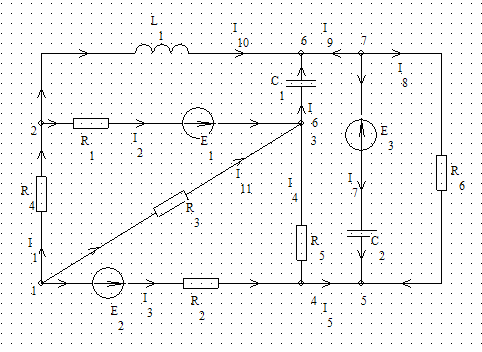
\includegraphics[height = 13\baselineskip]{assets/01-01-scheme-full.png}
		\caption{Задане електричне коло}
		\label{fig:01-scheme-full}
		\end{figure}
		
		Значення напруг та опорів у електричному колі наведені у табл.~\ref{tab:01-voltages} і~\ref{tab:01-resistances} відповідно.
		
		\begin{longtable}{lr}
			\toprule
				Джерело ЕРС & Напруга (\si{\volt})\\
			\midrule
			\endhead
			\bottomrule
			\caption{Значення напруг джерел ЕРС в даному електричному колі}
			\endfoot
			\label{tab:01-voltages}
			
			$E_1$ & 20\\
			$E_2$ & 24\\
			$E_3$ & 20\\
		\end{longtable}
		
		\begin{longtable}{lr}
			\toprule
				Резистор & Опір (\si{\ohm})\\
			\midrule
			\endhead
			\bottomrule
			\caption{Значення опорів в даному електричному колі}
			\endfoot
			\label{tab:01-resistances}
			
			$R_1$ & 30\\
			$R_2$ & 25\\
			$R_3$ & 30\\
			$R_4$ & 25\\
			$R_5$ & 20\\
			$R_6$ & 20\\
		\end{longtable}
		
		\subsection{Складення спрощеної схеми}
			За заданим електричним колом~(рис.~\ref{fig:01-scheme-full}) була складена спрощена схема~(рис.~\ref{fig:02-scheme-simplified}).
			
			\begin{figure}[!htbp]
			\centering
				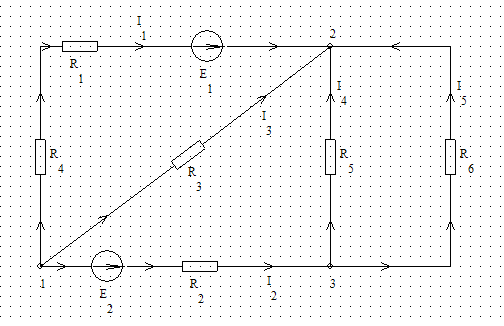
\includegraphics[height = 14\baselineskip]{assets/01-02-scheme-simplified.png}
			\caption{Спрощена схема}
			\label{fig:02-scheme-simplified}
			\end{figure}
	
		\subsection{Метод рівнянь Кірхгофа}
			Необхідно скласти систему рівнянь для розрахунку спрощеного кола за методом рівнянь Кірхгофа. Спочатку проаналізуємо електричне коло. Бачимо, що кількість вузлів~$q = 3$, а кількість гілок~$p = 5$. Отже, за першим законом Кірхгофа необхідно скласти $q - 1 = 2$ рівнянь; за другим законом Кірхгофа складається $p - (q - 1) = 3$~рівняння. Запишемо рівняння за першим законом Кірхгофа:
			\begin{IEEEeqnarray*}{rCl}
				I_1 + I_2 + I_3 &=& 0,\\
				-I_1 - I_3 - I_4 - I_5 &=& 0.
			\end{IEEEeqnarray*}
			За другим законом Кірхгофа:
			\begin{IEEEeqnarray*}{rCl}
				-I_1 \cdot \left( R_1 + R_4 \right) + I_3 \cdot R_3 &=& -E_1,\\
				I_3 \cdot R_3 - I_4 \cdot R_5 - I_2 \cdot R_2 &=& -E_2,\\
				-I_5 \cdot R_6 + I_4 \cdot R_5 &=& 0.
			\end{IEEEeqnarray*}
			
			Отримали систему:
			\begin{IEEEeqnarray*}{c}
				\left\{
					\begin{IEEEeqnarraybox}[
						\IEEEeqnarraystrutmode
						\IEEEeqnarraystrutsizeadd{2pt}{2pt}
					][c]{l}
						I_1 + I_2 + I_3 = 0,\\
						-I_1 - I_3 - I_4 - I_5 = 0,\\
						-I_1 \cdot \left( R_1 + R_4 \right) + I_3 \cdot R_3 = -E_1,\\
						I_3 \cdot R_3 - I_4 \cdot R_5 - I_2 \cdot R_2 = -E_2,\\
						-I_5 \cdot R_6 + I_4 \cdot R_5 = 0.
					\end{IEEEeqnarraybox}
				\right.
			\end{IEEEeqnarray*}
			
		\subsection{Метод контурних струмів}
			Визначимо напруги в контурі:
			\begin{IEEEeqnarray*}{l}
				E_{11} = -E_1 = \SI{-20}{\volt},\\
				E_{22} = -E_2 = \SI{-24}{\volt},\\
				E_{33} = \SI{0}{\volt}.
			\end{IEEEeqnarray*}
			
			Обчислимо опори:
			\begin{IEEEeqnarray*}{lll}
				\begin{IEEEeqnarraybox}{l}
				R_{11} = R_1 + R_4 + R_3 = \SI{85}{\ohm},\\
				% R_{12} = R_3 = \SI{30}{\ohm},\\
				R_{21} = R_3 = \SI{30}{\ohm},\\
				% R_{13} = \SI{0}{\ohm},\\
				R_{31} = \SI{0}{\ohm},
				\end{IEEEeqnarraybox}
				\quad
				\begin{IEEEeqnarraybox}{l}
				% R_{21} = R_3 = \SI{30}{\ohm},\\
				R_{12} = R_3 = \SI{30}{\ohm},\\
				R_{22} = R_3 + R_5 + R_2 = \SI{75}{\ohm},\\
				% R_{23} = -R_5 = \SI{-20}{\ohm},\\
				R_{32} = -R_5 = \SI{-20}{\ohm},
				\end{IEEEeqnarraybox}
				\quad
				\begin{IEEEeqnarraybox}{l}
				% R_{31} = \SI{0}{\ohm},\\
				R_{13} = \SI{0}{\ohm},\\
				R_{23} = -R_5 = \SI{-20}{\ohm},\\
				% R_{32} = -R_5 = \SI{-20}{\ohm},\\
				R_{33} = R_6 + R_5 = \SI{40}{\ohm}.
				\end{IEEEeqnarraybox}
			\end{IEEEeqnarray*}
			
			% Обчислимо опори:
			% \begin{IEEEeqnarray*}{l}
				% R_{11} = R_1 + R_4 + R_3 = \SI{85}{\ohm},\\
				% R_{12} = R_3 = \SI{30}{\ohm},\\
				% R_{13} = \SI{0}{\ohm},\\
				% R_{21} = R_3 = \SI{30}{\ohm},\\
				% R_{22} = R_3 + R_5 + R_2 = \SI{75}{\ohm},\\
				% R_{23} = -R_5 = \SI{-20}{\ohm},\\
				% R_{31} = \SI{0}{\ohm},\\
				% R_{32} = -R_5 = \SI{-20}{\ohm},\\
				% R_{33} = R_6 + R_5 = \SI{40}{\ohm},\\
			% \end{IEEEeqnarray*}
			
			Складаємо систему рівнянь за другим законом Кірхгофа:
			\begin{IEEEeqnarray*}{c}
				\left\{
					\begin{IEEEeqnarraybox}[
						\IEEEeqnarraystrutmode
						\IEEEeqnarraystrutsizeadd{2pt}{2pt}
					][c]{rCl}
						I_{11} \cdot R_{11} + I_{22} \cdot R_{12} + I_{33} \cdot R_{13} = E_{11},\\
						I_{11} \cdot R_{21} + I_{22} \cdot R_{22} + I_{33} \cdot R_{23} = E_{22},\\
						I_{11} \cdot R_{31} + I_{22} \cdot R_{32} + I_{33} \cdot R_{33} = E_{33}.
					\end{IEEEeqnarraybox}
				\right.
				=
				\left\{
					\begin{IEEEeqnarraybox}[
						\IEEEeqnarraystrutmode
						\IEEEeqnarraystrutsizeadd{2pt}{2pt}
					][c]{rCrCrCr}
						85 I_{11}  &+& 30 I_{22} &&            &=& -20,\\
						30 I_{11}  &+& 75 I_{22} &-& 20 I_{33} &=& -24,\\
						           &-& 20 I_{22} &+& 40 I_{33} &=& 0.
					\end{IEEEeqnarraybox}
				\right.
			\end{IEEEeqnarray*}
			
			Розв'язавши складену систему рівнянь отримали значення контурних струмів:
			\begin{IEEEeqnarray*}{rCl}
				I_{11} &=& \SI{-0.125405}{\ampere},\\
				I_{22} &=& \SI{-0.311351}{\ampere},\\
				I_{33} &=& \SI{-0.155675}{\ampere}.
			\end{IEEEeqnarray*}
			
			За значеннями контурних струмів обчислимо значення діючих:
			\begin{IEEEeqnarray*}{lClCr}
				I_1 &=& -I_{11}          &=& \SI{ 0.125405}{\ampere},\\
				I_2 &=& -I_{22}          &=& \SI{ 0.311351}{\ampere},\\
				I_3 &=& +I_{11} + I_{22} &=& \SI{-0.436757}{\ampere},\\
				I_4 &=& -I_{22} + I_{33} &=& \SI{ 0.155676}{\ampere},\\
				I_5 &=& -I_{33}          &=& \SI{ 0.155676}{\ampere}.
			\end{IEEEeqnarray*}
			
			% Виконаємо перевірку за рівнянням балансу потужностей. Для цього обчислимо потужності джерел та приймачів:
			% \begin{IEEEeqnarray*}{rCl}
				% \sum_{k = 1}^n I^2_k R_k
				% &=& {I_1}^2 \cdot R_4 + {I_1}^2 \cdot R_1 + {I_2}^2 \cdot R_2 + {I_3}^2 \cdot R_3 + {I_4}^2 \cdot R_5 + {I_5}^2 \cdot R_6 \\
				% &=& \num{0.393163} + \num{0.471795} + \num{2.423490} + \num{5.722690} + \num{0.484698} + \num{0.484698}\\
				% &=& \num{9.980540}.\\
				% \sum_{k = 1}^{n} E_k I_k
				% &=& E_1 \cdot I_1 + E_2 \cdot I_2\\
				% &=& \num{2.508108} + \num{7.783783}\\
				% &=& \num{10.291892}.
			% \end{IEEEeqnarray*}
			
			% Похибка~$\varepsilon = \num{0.311335}$.
		
		\subsection{Метод вузлових потенціалів}
			Приймемо потенціал третього вузла за нуль: $\varphi_3 = 0$, тоді рівняння для двох інших вузлів матимуть вигляд:
			\begin{IEEEeqnarray*}{rCl}
				\varphi_{1} \cdot G_{11} + \varphi_{2} \cdot G_{12} = I_{11},\\
				\varphi_{1} \cdot G_{21} + \varphi_{2} \cdot G_{22} = I_{22}.
			\end{IEEEeqnarray*}
			
			Обчислимо значення взаємних та вузлових провідностей:
			\begin{IEEEeqnarray*}{l}
			G_{11} = \frac{1}{R_1 + R_4} + \frac{1}{R_2} + \frac{1}{R_3}
			       = \SI{0.091515}{\siemens},\\[2\jot]
			G_{12} = -\frac{1}{R_1 + R_4} - \frac{1}{R_3}
			       =\SI{-0.051515}{\siemens},\\[2\jot]
			G_{22} = \frac{1}{R_1 + R_4} + \frac{1}{R_3} + \frac{1}{R_5} + \frac{1}{R_6}
			       = \SI{0.151515}{\siemens}.
			\end{IEEEeqnarray*}
			
			Обчислимо значення вузлових струмів:
			\begin{IEEEeqnarray*}{l}
			I_{11} = \frac{-E_1}{R_1 + R_4} - \frac{E_2}{R_2}
			       = \SI{-1.32364}{\ampere},\\[2\jot]
			I_{22} = \frac{E_1}{R_1 + R_4}
			       = \SI{0.36364}{\ampere}.
			\end{IEEEeqnarray*}
			
			Складаємо систему рівнянь за отриманими значеннями:
			\begin{IEEEeqnarray*}{c}
				\left\{
					\begin{IEEEeqnarraybox}[
						\IEEEeqnarraystrutmode
						\IEEEeqnarraystrutsizeadd{2pt}{2pt}
					][c]{rCrCr}
						\num{ 0.091515} \varphi_1 &-& \num{0.051515} \varphi_2 &=& \num{-1.32360},\\
						\num{-0.051515} \varphi_1 &-& \num{0.151520} \varphi_2 &=& \num{ 0.36364}.
					\end{IEEEeqnarraybox}
				\right.
			\end{IEEEeqnarray*}
			
			Після розв'язання системи рівнянь, отримали значення шуканих вузлових потенціалів:
			\begin{IEEEeqnarray*}{rCl}
				\varphi_1 &=& \num{-16.2160},\\
				\varphi_2 &=& \num{-03.1135},\\
				\varphi_3 &=& \num{0}.
			\end{IEEEeqnarray*}
			
			Обчислимо дійсні значення струмів за допомогою отриманих значень вузлових потенціалів:
			\begin{IEEEeqnarray*}{l}
				I_1 = \frac{\varphi_1 - \varphi_2 + E_1}{R_1 + R_4}
				    = \SI{ 0.125405}{\ampere},\\[2\jot]
				I_2 = \frac{\varphi_1 - \varphi_3 + E_2}{R_2}
				    = \SI{ 0.311351}{\ampere},\\[2\jot]
				I_3 = \frac{\varphi_1 - \varphi_2}{R_3}
				    = \SI{-0.436757}{\ampere},\\[2\jot]
				I_4 = \frac{\varphi_3 - \varphi_2}{R_3}
				    = \SI{ 0.155676}{\ampere},\\[2\jot]
				I_5 = \frac{\varphi_3 - \varphi_2}{R_3}
				    = \SI{ 0.155676}{\ampere}.
			\end{IEEEeqnarray*}
			
		\subsection{Перевірка за рівнянням балансу потужностей}
			Виконаємо перевірку за рівнянням балансу потужностей для результатів, отриманих при розрахунку \emph{методом контурних струмів}. Для цього обчислимо потужності джерел та приймачів:
			\begin{IEEEeqnarray*}{rCl}
				\sum_{k = 1}^n I^2_k R_k
				&=& {I_1}^2 \cdot R_4 + {I_1}^2 \cdot R_1 + {I_2}^2 \cdot R_2 + {I_3}^2 \cdot R_3 + {I_4}^2 \cdot R_5 + {I_5}^2 \cdot R_6 \\
				&=& \num{0.393163} + \num{0.471795} + \num{2.423490} + \num{5.722690} + \num{0.484698} + \num{0.484698}\\
				&=& \num{9.980540}.\\
				\sum_{k = 1}^{n} E_k I_k
				&=& E_1 \cdot I_1 + E_2 \cdot I_2\\
				&=& \num{2.508108} + \num{7.783783}\\
				&=& \num{10.291892}.
			\end{IEEEeqnarray*}
			Похибка~$\varepsilon = \num{0.311335}$.
			
			Виконаємо перевірку за рівнянням балансу потужностей для результатів, отриманих при розрахунку \emph{методом вузлових потенціалів}. Для цього обчислимо потужності джерел та приймачів:
			\begin{IEEEeqnarray*}{rCl}
				\sum_{k = 1}^n I^2_k R_k
				&=& {I_1}^2 \cdot R_4 + {I_1}^2 \cdot R_1 + {I_2}^2 \cdot R_2 + {I_3}^2 \cdot R_3 + {I_4}^2 \cdot R_5 + {I_5}^2 \cdot R_6 \\
				&=& \num{0.393160} + \num{0.471792} + \num{2.423486} + \num{5.722700} + \num{0.484700} + \num{0.484700}\\
				&=& \num{9.980540}.\\
				\sum_{k = 1}^{n} E_k I_k
				&=& E_1 \cdot I_1 + E_2 \cdot I_2\\
				&=& \num{2.508100} + \num{7.783775}\\
				&=& \num{10.291875}.
			\end{IEEEeqnarray*}
			Похибка~$\varepsilon = \num{0.311335}$.
			
		\subsection{Потенціальна діаграма}
			Потенціальна діаграма заданого контура зображена на рис.~\ref{fig:potential-diagram}.
			\begin{figure}[!htbp]
			\centering
				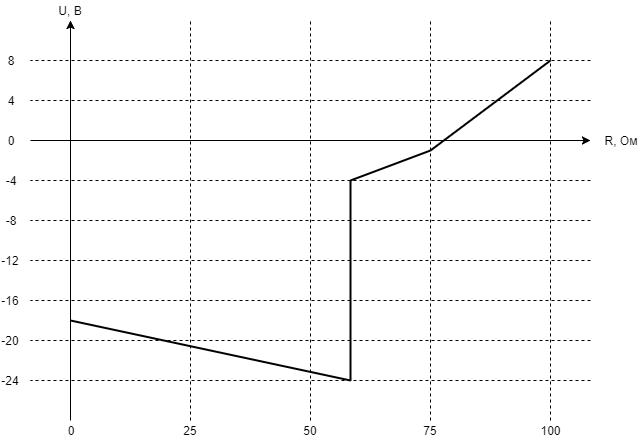
\includegraphics[width = \textwidth]{assets/01-03-diagram-potential.png}
			\caption{Потенціальна діаграма контура}
			\label{fig:potential-diagram}
			\end{figure}
			
	\section{Розрахунок лінійного електричного~кола синусоїдного~струму}
		Для виконання завдання необхідно:
		\begin{enumerate}
			\item Визначити значення напруг і струмів у всіх гілках кола.
			\item Перевірити точність виконаних розрахунків, скориставшись рівнянням балансу потужностей.
			\item Побудувати променеву векторну діаграму струмів і топографічну векторну діаграму напруг кола.
			\item Записати миттєві значення всіх струмів і напруг.
		\end{enumerate}
		
		Задане електричне кого зображене на рис.~\ref{fig:02-01-scheme-full}.
		\begin{figure}[!htbp]
		\centering
			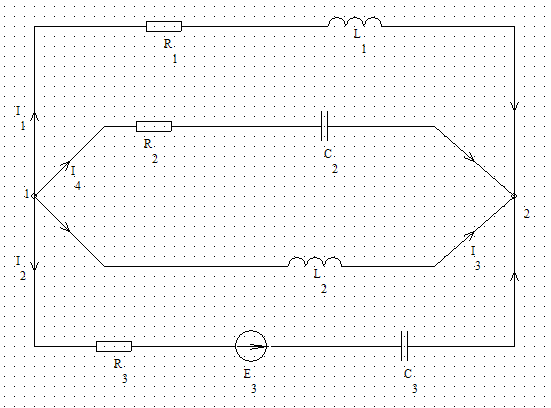
\includegraphics[height = 12\baselineskip]{assets/02-01-scheme-full.png}
		\caption{Задане електричне коло}
		\label{fig:02-01-scheme-full}
		\end{figure}
		
		При виконанні розрахунків вважати, що $\varphi = 400$, $\omega = 2 \pi \varphi = 2513$. Напруга джерела ЕРС~$E_{3} = \SI{90}{\volt}$. Значення параметрів заданого електричного кола наведені у табл~\ref{tab:02-resistance-values}, \ref{tab:02-induction-values}, \ref{tab:02-capacity-values}.
		
		\begin{longtable}{lr}
			\toprule
				Резистор & Опір (\si{\ohm})\\
			\midrule
			\endhead
			\bottomrule
			\caption{Значення опорів резисторів для заданого електричного кола}
			\endfoot
			\label{tab:02-resistance-values}
			
			$R_1$ & \num{130}\\
			$R_2$ & \num{115}\\
			$R_3$ & \num{110}\\
		\end{longtable}
		
		\begin{longtable}{lr}
			\toprule
				Котушка & Індуктивність (\si{\milli\henry})\\
			\midrule
			\endhead
			\bottomrule
			\caption{Значення індуктивностей котушок для заданого електричного кола}
			\endfoot
			\label{tab:02-induction-values}
			
			$L_1$ & \num{42}\\
			$L_2$ & \num{47}\\
			$L_3$ & \num{43}\\
		\end{longtable}
		
		\begin{longtable}{lr}
			\toprule
				Конденсатор & Ємність (\si{\micro\farad})\\
			\midrule
			\endhead
			\bottomrule
			\caption{Значення ємностей конденсаторів для заданого електричного кола}
			\endfoot
			\label{tab:02-capacity-values}
			
			$C_1$ & \num{2.7}\\
			$C_2$ & \num{2.2}\\
			$C_3$ & \num{2.9}\\
		\end{longtable}
		
		\subsection{Визначення напруг і струмів}
			Для розрахунку даного кола використаємо \emph{метод контурних струмів}. Спочатку знайдемо опори кожної з гілок електричного кола:
			\begin{IEEEeqnarray*}{l}
				Z_1 = R_1 + j \cdot \omega \cdot L_1
				    = 130 + j \cdot 2513 \cdot 0{,}042
					= 130 + j \cdot 105{,}6,\\[2\jot]
				Z_2 = R_3 + j \cdot \frac{-1}{\omega \cdot C_3}
				    = 110 + j \cdot \frac{-1}{2513 \cdot \num{2.9e-6}}
					= 110 - j \cdot 137{,}2,\\[2\jot]
				Z_3 = j \cdot \omega \cdot L_2
				    = j \cdot 2513 \cdot 0{,}047
					= j \cdot 118{,}1,\\[2\jot]
				Z_4 = R_2 + j \cdot \frac{-1}{\omega \cdot C_2}
				    = 115 + j \cdot \frac{-1}{2513 \cdot \num{2.2e-6}}
					= j \cdot 118{,}1.
			\end{IEEEeqnarray*}
			
			Знайдемо контурні опори:
			\begin{IEEEeqnarray*}{lll}
				\begin{IEEEeqnarraybox}[
					\IEEEeqnarraystrutmode
					\IEEEeqnarraystrutsizeadd{2pt}{2pt}
				][c]{l}
					Z_{11} = Z_1 + Z_4 = 245 - j \cdot 75{,}3,\\
					Z_{21} = 0,\\
					Z_{31} = -Z_4 = -115 + j \cdot 180{,}9,
				\end{IEEEeqnarraybox}
				\quad
				\begin{IEEEeqnarraybox}[
					\IEEEeqnarraystrutmode
					\IEEEeqnarraystrutsizeadd{2pt}{2pt}
				][c]{l}
					Z_{12} = 0,\\
					Z_{22} = Z_2 + Z_3 = 110 - j \cdot 19{,}08,\\
					Z_{32} = Z_3 = j \cdot 118{,}1,
				\end{IEEEeqnarraybox}
				\quad
				\begin{IEEEeqnarraybox}[
					\IEEEeqnarraystrutmode
					\IEEEeqnarraystrutsizeadd{2pt}{2pt}
				][c]{l}
					Z_{13} = -Z_4 = -115 + j \cdot 180{,}9,\\
					Z_{23} = Z_3 = j \cdot 118{,}1,\\
					Z_{33} = Z_4 + Z_3 = 115 - j \cdot 62{,}73.
				\end{IEEEeqnarraybox}
			\end{IEEEeqnarray*}
			
			Знайдемо напруги:
			\begin{IEEEeqnarray*}{l}
				E_{11} = \SI{0}{\volt},\\
				E_{22} = E_3 = \SI{90}{\volt},\\
				E_{33} = \SI{0}{\volt},\\
			\end{IEEEeqnarray*}
			
			Складаємо систему рівнянь для контурних струмів:
			\begin{IEEEeqnarray*}{c}
				\left\{
					\begin{IEEEeqnarraybox}[
						\IEEEeqnarraystrutmode
						\IEEEeqnarraystrutsizeadd{2pt}{2pt}
					][c]{rCl}
						I_{11} \cdot Z_{11} + I_{22} \cdot Z_{12} + I_{33} \cdot Z_{13} = E_{11},\\
						I_{11} \cdot Z_{21} + I_{22} \cdot Z_{22} + I_{33} \cdot Z_{23} = E_{22},\\
						I_{11} \cdot Z_{31} + I_{22} \cdot Z_{32} + I_{33} \cdot Z_{33} = E_{33}.
					\end{IEEEeqnarraybox}
				\right.
				% =
				% \left\{
					% \begin{IEEEeqnarraybox}[
						% \IEEEeqnarraystrutmode
						% \IEEEeqnarraystrutsizeadd{2pt}{2pt}
					% ][c]{rCrCrCr}
						% 85 I_{11}  &+& 30 I_{22} &&            &=& -20,\\
						% 30 I_{11}  &+& 75 I_{22} &-& 20 I_{33} &=& -24,\\
						           % &-& 20 I_{22} &+& 40 I_{33} &=& 0.
					% \end{IEEEeqnarraybox}
				% \right.
			\end{IEEEeqnarray*}
			
			Підставимо знайдені значення у складену систему:
			\begin{IEEEeqnarray*}{c}
				\left\{
					\begin{IEEEeqnarraybox}[
						\IEEEeqnarraystrutmode
						\IEEEeqnarraystrutsizeadd{2pt}{2pt}
					][c]{l}
						\left(245 - j \cdot 75{,}3\right) \cdot I_{11} + \left( -115 + j \cdot 180{,}9 \right) \cdot I_{33} = 0,\\
						\left(110 - j \cdot 19{,}08\right) \cdot I_{22} -  \left(j \cdot 118{,}1 \right) \cdot I_{33} = 90,\\
						\left( -115 + j \cdot 180{,}9 \right) \cdot I_{11} + \left( j \cdot 118{,}1 \right) \cdot I_{22} + \left( 115 - j \cdot 62{,}73 \right) \cdot I_{33} = 0.
					\end{IEEEeqnarraybox}
				\right.
			\end{IEEEeqnarray*}
			
			Розв'язавши отриману систему рівнянь отримали:
			\begin{IEEEeqnarray*}{l}
				I_{11} = -0{,}2279 - j \cdot 0{,}1425,\\
				I_{22} =  0{,}4572 - j \cdot 0{,}1831,\\
				I_{33} = -0{,}0967 - j \cdot 0{,}13066.
			\end{IEEEeqnarray*}
			
			Знайдемо комплексні струми за знайденими контурними струмами:
			\begin{IEEEeqnarray*}{l}
				I_1 = I_{11} = -0{,}2279 - j \cdot 0{,}1425,\\
				I_2 = I_{22} =  0{,}4572 - j \cdot 0{,}1831,\\
				I_3 = -I_{22} - I_{33} = -0{,}3605 + j \cdot 0{,}1234,\\
				I_4 = -I_{11} + I_{33} =  0{,}1312 + j \cdot 0{,}1640.
			\end{IEEEeqnarray*}
			
		\subsection{Перевірка за рівнянням балансу потужностей}
			Виконаємо перевірку за рівнянням балансу потужностей:
			% \sum_{k = 1}^n I^2_k R_k
			% \sum_{k = 1}^{n} E_k I_k
			
			\begin{IEEEeqnarray*}{l}
				\sum S_{k \text{дж}} =
				\abs{I_1}^2 \cdot R_1
				+ \abs{I_1}^2 \cdot j \omega L_1
				+ \abs{I_2}^2 \cdot R_3
				- \abs{I_2}^2 \cdot \frac{j}{\omega \cdot C_3} \qquad \\
				\IEEEeqnarraymulticol{1}{r}{ +\> \abs{I_3}^2 \cdot j \omega L_2
				+ \abs{I_4}^2 \cdot R_2
				- \abs{I_4}^2 \cdot \frac{j}{\omega \cdot C_2}.}
			\end{IEEEeqnarray*}
			
			Виконуємо обчислення:
			\begin{IEEEeqnarray*}{l}
				0{,}01117 + j \cdot 0{,}00907 + 0{,}7516 - j \cdot 0{,}9375 + j \cdot 0{,}7949 \hspace*{3em} \\
				\IEEEeqnarraymulticol{1}{r}{ +\> \num{8{,}009e-5} - j \cdot 0{,}000126 = 0{,}7628 - j \cdot 0{,}1336.}
			\end{IEEEeqnarray*}
			
			% \begin{IEEEeqnarray*}{rCCl} % FIXME
			% \sum_{k = 1}^n I^2_k R_k &=& &
			%	&=& \abs{I_1}^2 \cdot R_1
				% \abs{I_1}^2 \cdot R_1
				% + \abs{I_1}^2 \cdot j \omega L_1
				% + \abs{I_2}^2 \cdot R_3
				% - \abs{I_2}^2 \cdot \frac{j}{\omega \cdot C_3}\\
				% &&+& \abs{I_3}^2 \cdot j \omega L_2
				% + \abs{I_4}^2 \cdot R_2
				% - \abs{I_4}^2 \cdot \frac{j}{\omega \cdot C_2} \\
				% &=&& 0{,}01117 + j \cdot 0{,}00907 + 0{,}7516 - j \cdot 0{,}9375 + j \cdot 0{,}7949 + \num{8{,}009e-5} - j \cdot 0{,}000126\\
				% &=&& 0{,}7628 - j \cdot 0{,}1336.
			% \end{IEEEeqnarray*}
			
			Також:
			\begin{IEEEeqnarray*}{l}
				\sum S_{k \text{сп}} = \left( \Re(I_2) - j \cdot \Im(I_2) \right) \cdot E_3 = 0{,}7628 - j \cdot 7,4.
			\end{IEEEeqnarray*}
			
			Похибка~$\varepsilon = 0{,}7628 - j \cdot 0{,}1336 – 0{,}7628 - j \cdot 7{,}4 = j \cdot 7{,}2664$.
			
		\subsection{Визначення дійсних і миттєвих значень}
			\subsubsection{Струмів}
				Знайдемо амплітудні значення струмів:
				\begin{IEEEeqnarray*}{l}
					I_{1m} = \sqrt{0{,}2279^2 + 0{,}1425^2} = 0{,}2687,\\[2\jot]
					I_{2m} = \sqrt{0{,}4572^2 + 0{,}1831^2} = 0{,}4925,\\[2\jot]
					I_{3m} = \sqrt{0{,}3605^2 + 0{,}1234^2} = 0{,}4043,\\[2\jot]
					I_{4m} = \sqrt{0{,}1312^2 + 0{,}1640^2} = 0{,}2100.
				\end{IEEEeqnarray*}
				
				Обчислимо значення початкових фаз:
				\begin{IEEEeqnarray*}{l}
					\psi_{i_1} = \arctg \left( \frac{0{,}1425}{0{,}2279} \right) = 0{,}5587,\\[2\jot]
					\psi_{i_2} = \arctg \left( \frac{0{,}1831}{0{,}4572} \right) = 0{,}3809,\\[2\jot]
					\psi_{i_3} = \arctg \left( \frac{0{,}1234}{0{,}3605} \right) = 0{,}3298,\\[2\jot]
					\psi_{i_4} = \arctg \left( \frac{0{,}1640}{0{,}1312} \right) = 0{,}8960.
				\end{IEEEeqnarray*}
				
				Обчислимо значення діючих струмів за формулою~\eqref{eq:current-imaginary-to-real}.
				
				\begin{equation}
				\label{eq:current-imaginary-to-real}
					I_i = \frac{I_{im}}{\sqrt{2}}.
				\end{equation}
				
				Виконуємо обчислення:
				\begin{IEEEeqnarray*}{l}
					I_1 = \frac{I_{1m}}{\sqrt{2}} = \frac{0{,}2687}{1{,}4142} = 0{,}1900,\\[2\jot]
					I_2 = \frac{I_{2m}}{\sqrt{2}} = \frac{0{,}4925}{1{,}4142} = 0{,}3482,\\[2\jot]
					I_3 = \frac{I_{3m}}{\sqrt{2}} = \frac{0{,}4043}{1{,}4142} = 0{,}2858,\\[2\jot]
					I_4 = \frac{I_{4m}}{\sqrt{2}} = \frac{0{,}2100}{1{,}4142} = 0{,}1484.
				\end{IEEEeqnarray*}
				
				Обчислимо миттєві струми за формулою~\eqref{eq:current-real-to-measurable}.
				
				\begin{equation}
				\label{eq:current-real-to-measurable}
					i = I_{im} \sin \left( \omega t + \Psi_i \right).
				\end{equation}
				
				Виконуємо обчислення:
				\begin{IEEEeqnarray*}{l}
					i_1 = 0{,}1900 \cdot \sin \left( 2513 t + 0{,}5587 \right),\\
					i_2 = 0{,}3448 \cdot \sin \left( 2513 t + 0{,}3809 \right),\\
					i_3 = 0{,}2858 \cdot \sin \left( 2513 t + 0{,}3298 \right),\\
					i_4 = 0{,}1484 \cdot \sin \left( 2513 t + 0{,}8960 \right).
				\end{IEEEeqnarray*}
				
			\subsubsection{Напруг}
				Знайдемо амплітудні значення напруг:
				\begin{IEEEeqnarray*}{l}
					U_{1m} = \sqrt{14{,}5790^2 + 42{,}5912^2} = 45{,}0161,\\[2\jot]
					U_{2m} = \sqrt{75{,}4133^2 + 42{,}5868^2} = 86{,}6071,\\[2\jot]
					U_{3m} = \sqrt{14{,}5735^2 + 42{,}5750^2} = 45{,}0001,\\[2\jot]
					U_{4m} = \sqrt{14{,}5796^2 + 42{,}5940^2} = 45{,}0201.
				\end{IEEEeqnarray*}
				
				Обчислимо значення початкових фаз:
				\begin{IEEEeqnarray*}{l}
					\psi_{u_1} = \arctg \left( \frac{42{,}5912}{14{,}579} \right) = 1{,}2409,\\[2\jot]
					\psi_{u_2} = \arctg \left( \frac{42{,}5868}{75{,}4133} \right) = 0{,}5140,\\[2\jot]
					\psi_{u_3} = \arctg \left( \frac{42{,}5750}{14{,}5735} \right) = 1{,}2409,\\[2\jot]
					\psi_{u_4} = \arctg \left( \frac{42{,}5940}{14{,}5796} \right) = 1{,}2410.
				\end{IEEEeqnarray*}
				
				Обчислимо значення діючих напруг:
				\begin{IEEEeqnarray*}{l}
					U_1 = \frac{U_{1m}}{\sqrt{2}} = \frac{45{,}0161}{1{,}4142} = 31{,}8314,\\[2\jot]
					U_2 = \frac{U_{2m}}{\sqrt{2}} = \frac{86{,}6071}{1{,}4142} = 61{,}2410,\\[2\jot]
					U_3 = \frac{U_{3m}}{\sqrt{2}} = \frac{45{,}0001}{1{,}4142} = 31{,}8201,\\[2\jot]
					U_4 = \frac{U_{4m}}{\sqrt{2}} = \frac{45{,}0201}{1{,}4142} = 31{,}8343.
				\end{IEEEeqnarray*}
				
				Обчислимо значення миттєвих напруг:
				\begin{IEEEeqnarray*}{l}
					u_1 = 45{,}0161 \cdot \sin \left( 2513 t + 1{,}2409\right),\\
					u_2 = 86{,}6071 \cdot \sin \left( 2513 t + 0{,}5140\right),\\
					u_3 = 45{,}0001 \cdot \sin \left( 2513 t + 1{,}2409\right),\\
					u_4 = 45{,}0201 \cdot \sin \left( 2513 t + 1{,}2410\right).
				\end{IEEEeqnarray*}
		\subsection{Діаграми}
			Векторна діаграма струмів зображена на рис.~\ref{fig:02-03-diagram-currents}. Топографічна діаграма напруг зображена на рис.~\ref{fig:02-04-diagram-voltages}.
			
			\begin{figure}[!htbp]
			\centering
				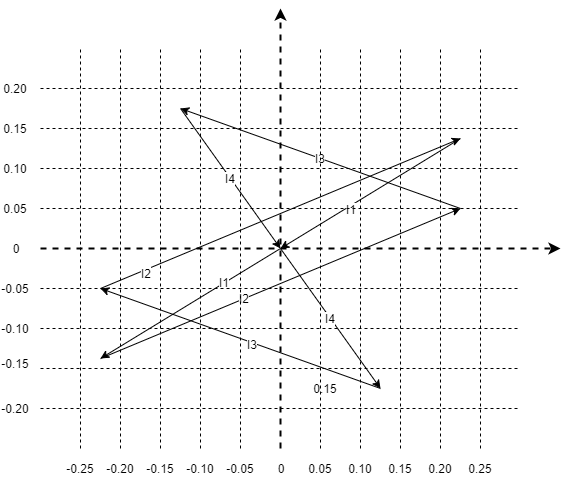
\includegraphics[width = 110mm]{assets/02-03-diagram-currents.png}
			\caption{Векторна діаграма струмів}
			\label{fig:02-03-diagram-currents}
			\end{figure}
			
			\begin{figure}[!htbp]
			\centering
				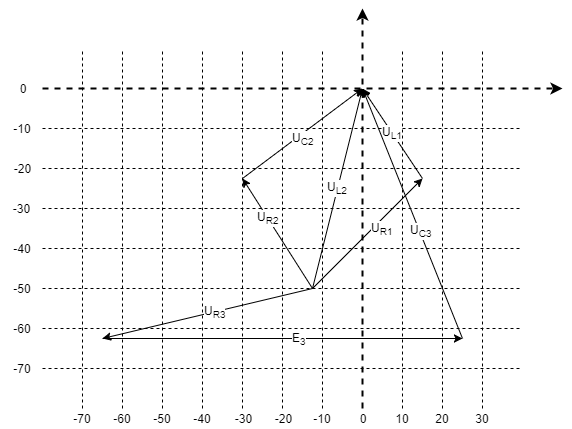
\includegraphics[width = 110mm]{assets/02-04-diagram-voltages.png}
			\caption{Потенціальна діаграма контура}
			\label{fig:02-04-diagram-voltages}
			\end{figure}
\end{document}